\graphicspath{{./figures/}}

\section{Problem Statement}

The initial problem statement was simply to design a communication system for a \mbox{PocketQube}, with focus on the ground station. As this is relatively broad, investigation of existing balloon-satellite systems, as well as the launch for this specific PocketQube, was done. An additional requirement that the GS should also be capable of receiving information from commercial \textit{radiosondes} (atmospheric telemetry devices) was also given. The specifications of existing radiosondes is therefore used as a reference, both for the new system's requirements, and as a consideration for system integration.

\begin{figure}[!htb]
  \centering
  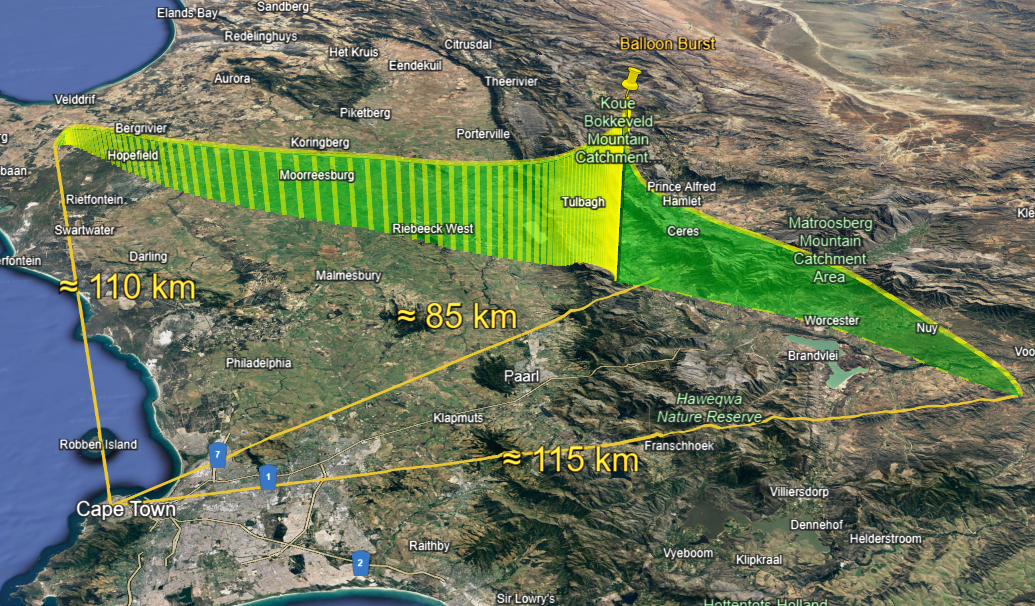
\includegraphics[width=0.72\textwidth]{balloon_path_3d}
  \caption{Predicted Balloon Path and Distances}
  \label{fig:balloon_path}
\end{figure}

High-altitude balloons can drift to a height as much as 30 km above sea level, and can drift as far as 200 km from launch \cite{site-weatherWeatherBalloons}. As mentioned, this project's launch is planned to be near Saldanha Airfield. Using the \textit{HabHub} path predictor \cite{site-habHub} on a day where the balloon travels far in-land, a launch from the airfield results in the path as in Figure \ref{fig:balloon_path}. From Cape Town, this is a maximum straight line distance of around 115 km. 

A ground station should maintain a reliable wireless link with a satellite to enable continuous communication and real-time telemetry. Since most radiosondes are simply uni-directional "downlink" devices, this should be a priority, however the GS should also be capable of bi-directional communication, in order to issue commands to the satellite.